\section{Riemann and the Reinvention of Integration (1854)}

\subsection{From Intuition to Rigor: Riemann’s Redefinition of Integration}

With Cauchy’s rigorous foundation of limits and continuity in place, the next major challenge in calculus was \textbf{integration}. While Newton and Leibniz had established integration as the inverse of differentiation, their definitions still relied on intuitive notions of infinitesimals and summation. Cauchy had already moved away from infinitesimals in his definition of continuity, so naturally, the next step was to redefine integration in a similarly rigorous way.  

Enter \textbf{Bernhard Riemann}.  

Riemann wasn’t just interested in making integration rigorous—he wanted to make it general. He sought to answer a fundamental question:  

\begin{quote}
What does it actually mean to compute the area under a curve?
\end{quote}

Before his work, integration was understood as summing infinitely small slices of a function’s graph. This worked well for “nice” functions, but as mathematicians began encountering more exotic, erratic functions, it became clear that the old methods were not sufficient. \textbf{Some functions simply refused to behave.}  

To solve this, Riemann introduced a new approach: defining integration in terms of \textbf{limits of sums}, not infinitesimals.  

\subsection{Riemann Sums: Approximating Area Through Partitions}

Riemann’s key insight was that the \textbf{integral of a function over an interval} could be understood as the limit of finite sums of function values over smaller and smaller partitions of that interval.  

Mathematically, he defined the \textbf{Riemann sum} as:  

\[
S = \sum_{i=1}^{n} f(x_i^*) \Delta x_i
\]

where:  
\begin{itemize}
    \item The interval \([a, b]\) is divided into \textbf{subintervals} \([x_{i-1}, x_i]\), each of width \( \Delta x_i = x_i - x_{i-1} \).  
    \item A representative sample point \( x_i^* \) is chosen from each subinterval.  
    \item The function value at \( x_i^* \) is multiplied by the subinterval width to approximate the area of each strip.  
\end{itemize}

\begin{center}
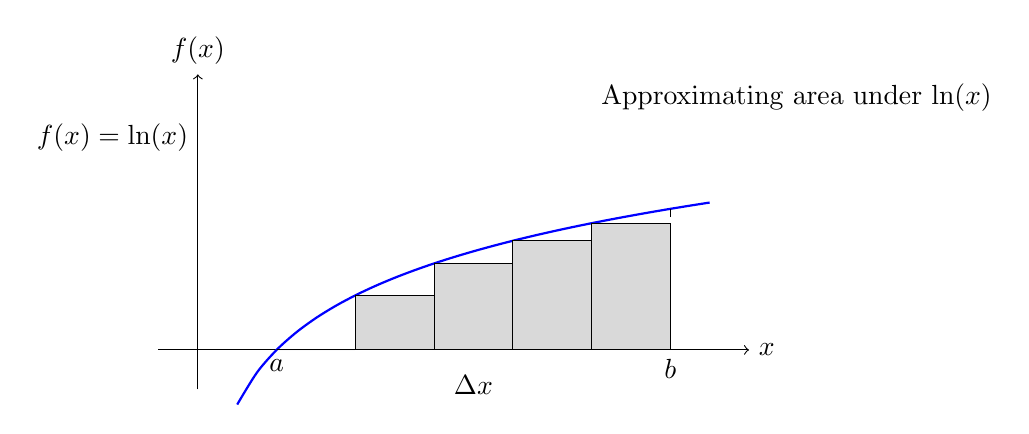
\begin{tikzpicture}
    % Draw axes
    \draw[->] (-0.5,0) -- (7,0) node[right] {\( x \)};
    \draw[->] (0,-0.5) -- (0,3.5) node[above] {\( f(x) \)};
    
    % Function curve: natural logarithm
    \draw[thick, blue, domain=0.5:6.5, smooth] plot (\x, {ln(\x)});
    
    % Interval [a, b]
    \node[below] at (1,0) {\( a \)};
    \node[below] at (6,0) {\( b \)};
    
    % Vertical dashed lines for subintervals
    \foreach \x in {1,2,3,4,5,6} {
        \draw[dashed] (\x,0) -- (\x,{ln(\x)});
    }

    % Rectangles (Riemann sum representation)
    \foreach \x in {1,2,3,4,5} {
        \pgfmathsetmacro\height{ln(\x)}
        \draw[fill=gray!30] (\x,0) rectangle (\x+1,\height);
    }

    % Labels
    \node[below] at (3.5,-0.2) {\( \Delta x \)};
    \node[left] at (0,2.7) {\( f(x) = \ln(x) \)};
    
    % Text description
    \node[right] at (5,3.2) {Approximating area under \( \ln(x) \)};
\end{tikzpicture}
\end{center}


By taking the \textbf{limit as the number of subintervals approaches infinity} (while the width of each subinterval shrinks to zero), the sum converges to a well-defined value—this is the \textbf{Riemann integral}:  

\[
\int_a^b f(x) \,dx = \lim_{n \to \infty} \sum_{i=1}^{n} f(x_i^*) \Delta x_i
\]

This formalization replaced the vague notion of “summing infinitely small quantities” with a \textbf{clear limit process}, ensuring that integration was built on the same solid foundations as differentiation.  







\begin{figure}[H]
\centering
\begin{tikzpicture}
\matrix[matrix of nodes, column sep=1.2cm, row sep=1.2cm] {
% Top-left: 2 rectangles
\node {
  \begin{tikzpicture}[scale=0.6]
    \draw[->] (-0.5,0) -- (7,0) node[right] {\(x\)};
    \draw[->] (0,-0.5) -- (0,3.5) node[above] {\(f(x)\)};
    \draw[thick, blue, domain=1:6.2, smooth] plot (\x, {ln(\x)});
    \foreach \x in {1,3.5} {
        \pgfmathsetmacro\h{ln(\x)}
        \draw[fill=gray!30] (\x,0) rectangle ({\x+2.5}, \h);
    }
    \node at (3,-0.8) {\scriptsize 2 rectangles};
  \end{tikzpicture}
}; &
% Top-right: 3 rectangles
\node {
  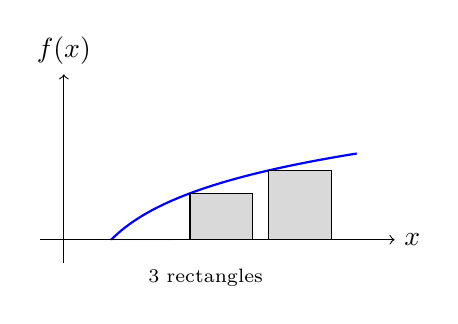
\begin{tikzpicture}[scale=0.6]
    \draw[->] (-0.5,0) -- (7,0) node[right] {\(x\)};
    \draw[->] (0,-0.5) -- (0,3.5) node[above] {\(f(x)\)};
    \draw[thick, blue, domain=1:6.2, smooth] plot (\x, {ln(\x)});
    \foreach \x in {1,2.67,4.33} {
        \pgfmathsetmacro\h{ln(\x)}
        \draw[fill=gray!30] (\x,0) rectangle ({\x+1.33}, \h);
    }
    \node at (3,-0.8) {\scriptsize 3 rectangles};
  \end{tikzpicture}
}; \\
% Bottom-left: 5 rectangles
\node {
  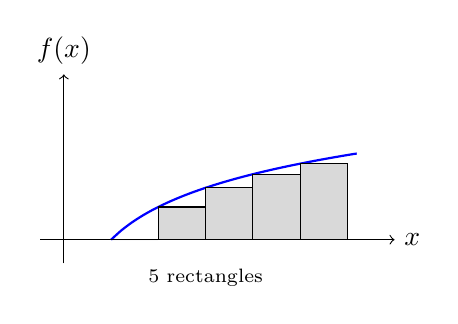
\begin{tikzpicture}[scale=0.6]
    \draw[->] (-0.5,0) -- (7,0) node[right] {\(x\)};
    \draw[->] (0,-0.5) -- (0,3.5) node[above] {\(f(x)\)};
    \draw[thick, blue, domain=1:6.2, smooth] plot (\x, {ln(\x)});
    \foreach \x in {1,2,3,4,5} {
        \pgfmathsetmacro\h{ln(\x)}
        \draw[fill=gray!30] (\x,0) rectangle ({\x+1}, \h);
    }
    \node at (3,-0.8) {\scriptsize 5 rectangles};
  \end{tikzpicture}
}; &
% Bottom-right: 10 rectangles
\node {
  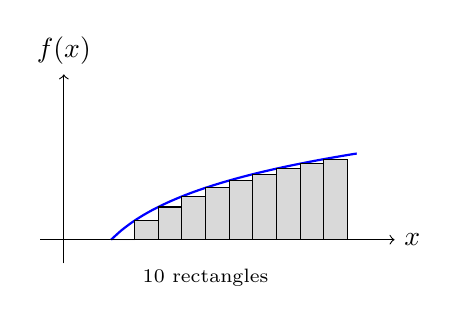
\begin{tikzpicture}[scale=0.6]
    \draw[->] (-0.5,0) -- (7,0) node[right] {\(x\)};
    \draw[->] (0,-0.5) -- (0,3.5) node[above] {\(f(x)\)};
    \draw[thick, blue, domain=1:6.2, smooth] plot (\x, {ln(\x)});
    \foreach \x in {1,1.5,...,5.5} {
        \pgfmathsetmacro\h{ln(\x)}
        \draw[fill=gray!30] (\x,0) rectangle ({\x+0.5}, \h);
    }
    \node at (3,-0.8) {\scriptsize 10 rectangles};
  \end{tikzpicture}
}; \\
};
\end{tikzpicture}
\caption{Left-endpoint Riemann sums: as the number of rectangles increases, the approximation of the area under \( \ln(x) \) becomes more accurate.}
\end{figure}




\subsection{Riemann’s Take on Kepler: Sweeping Areas by Limit}

So far, we’ve seen Kepler’s Second Law explained three ways:

\begin{itemize}
  \item \textbf{Kepler:} Geometric areas via exhaustion — sweeping out triangles like clockwork.
  \item \textbf{Leibniz:} Infinitesimal wedges adding up to a symbolic integral.
  \item \textbf{Newton:} Equal-area triangles in equal time, arguing from geometry and centripetal force.
\end{itemize}

But what if you were Riemann?

Then you'd approach Kepler’s area law the same way you approached integration itself: as a limit of finite approximations. Instead of infinitesimals or triangle tilings, you would partition time into small intervals, calculate the area swept out in each, and take the limit as the intervals shrink.

\subsubsection*{Kepler’s Law as a Riemann Sum}

Divide the time interval \([0, T]\) into \(n\) small subintervals of width \( \Delta t_i \), and suppose the planet’s position at time \(t_i\) is given in polar coordinates by \( (r_i, \theta_i) \). The area swept during a short interval is approximately a triangle:

\[
\Delta A_i \approx \frac{1}{2} r_i^2 \Delta \theta_i
\]

Then the total area swept becomes:

\[
A_n = \sum_{i=1}^n \frac{1}{2} r_i^2 \Delta \theta_i
\]

This is a \textbf{Riemann sum}. And in the limit as the time intervals become arbitrarily small:

\[
\boxed{
\lim_{n \to \infty} \sum_{i=1}^n \frac{1}{2} r_i^2 \Delta \theta_i = \int_0^T \frac{1}{2} r(t)^2 \, \frac{d\theta}{dt} \, dt
}
\]

This is precisely the integral that Leibniz arrived at using infinitesimals — but now grounded in Riemann’s rigorous theory of limits.

\subsubsection*{From Orbit to Integration}

In other words: \textbf{Kepler’s area law becomes a Riemann integral}.

It’s no longer just a geometric pattern or a philosophical gesture about infinitesimals — it becomes a computable quantity built from finite approximations. Riemann gave us the tools to make planetary motion not just visual, but verifiable.

\begin{quote}
What Newton tiled with triangles and Leibniz imagined with infinitesimals, Riemann measured — one limit at a time.
\end{quote}


\begin{figure}[H]
\centering
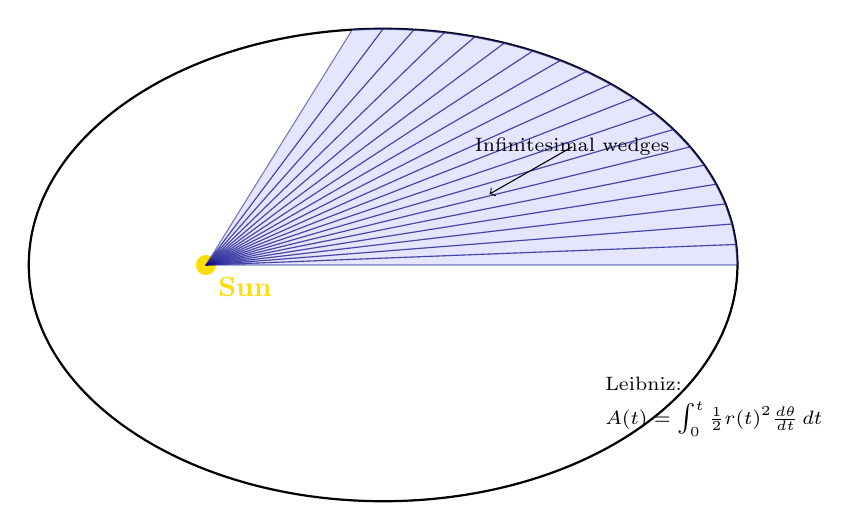
\begin{tikzpicture}[scale=3]

  % Elliptical orbit
  \draw[thick] (0,0) ellipse (1.5 and 1);

  % Sun at one focus
  \filldraw[yellow!80!orange] (-0.75,0) circle (0.04) node[below right=1pt] {\textbf{Sun}};

  % Draw infinitesimal wedges (thin triangles)
  \foreach \a in {0,5,...,90} {
    \draw[blue!50!black, fill=blue!20, opacity=0.5] 
      (-0.75,0) -- 
      ({1.5*cos(\a)}, {1*sin(\a)}) -- 
      ({1.5*cos(\a+5)}, {1*sin(\a+5)}) -- cycle;
  }

  % Label for wedge integration
  \node at (0.8,0.5) {\scriptsize Infinitesimal wedges};
  \draw[->] (0.8,0.5) -- (0.45,0.3);

  % Equation annotation (text only to avoid math nesting issues in nodes)
  \node[align=left] at (1.4,-0.6) {\scriptsize Leibniz: \\ \scriptsize $A(t) = \int_0^t \frac{1}{2} r(t)^2 \frac{d\theta}{dt} \, dt$};

\end{tikzpicture}
\caption{Here’s a visualization to contrast with Kepler’s geometric conception: Leibniz’s interpretation of area via infinitesimal wedges. Each thin triangle (or wedge) represents a tiny contribution to the total area swept out over time — just as Leibniz would have visualized it using his calculus notation: \( A(t) = \int_0^t \frac{1}{2} r(t)^2 \, \frac{d\theta}{dt} \, dt \). Whereas Kepler reasoned from equal areas traced out over equal times using exhaustion, Leibniz saw those same areas as the result of continuously accumulating infinitesimals. This view laid the foundation for how modern physics computes orbits, dynamics, and motion from first principles.}
\end{figure}



\subsection{The Power and Limitations of Riemann Integration}

Riemann’s definition worked beautifully for most functions encountered in classical mathematics. It was robust, logically consistent, and easy to apply to well-behaved functions. However, as analysis progressed, mathematicians began discovering functions that challenged even Riemann’s framework.  

Some functions were so irregular that \textbf{their Riemann sums never stabilized}—their partitions oscillated wildly, refusing to settle on a single area. This raised an uncomfortable question:  

\begin{quote}
Could a function be so badly behaved that it wasn’t integrable at all?
\end{quote}

Riemann had unknowingly opened a Pandora’s box. His definition worked, but only under certain conditions. What about the exceptions? What about functions that weren’t smooth, or even continuous?  

This realization led mathematicians to rethink the very nature of functions, pushing analysis beyond mere computation and into the realm of logical precision.  

And so, the field of \textbf{real analysis} was born.  


\begin{figure}[H]
    \centering
    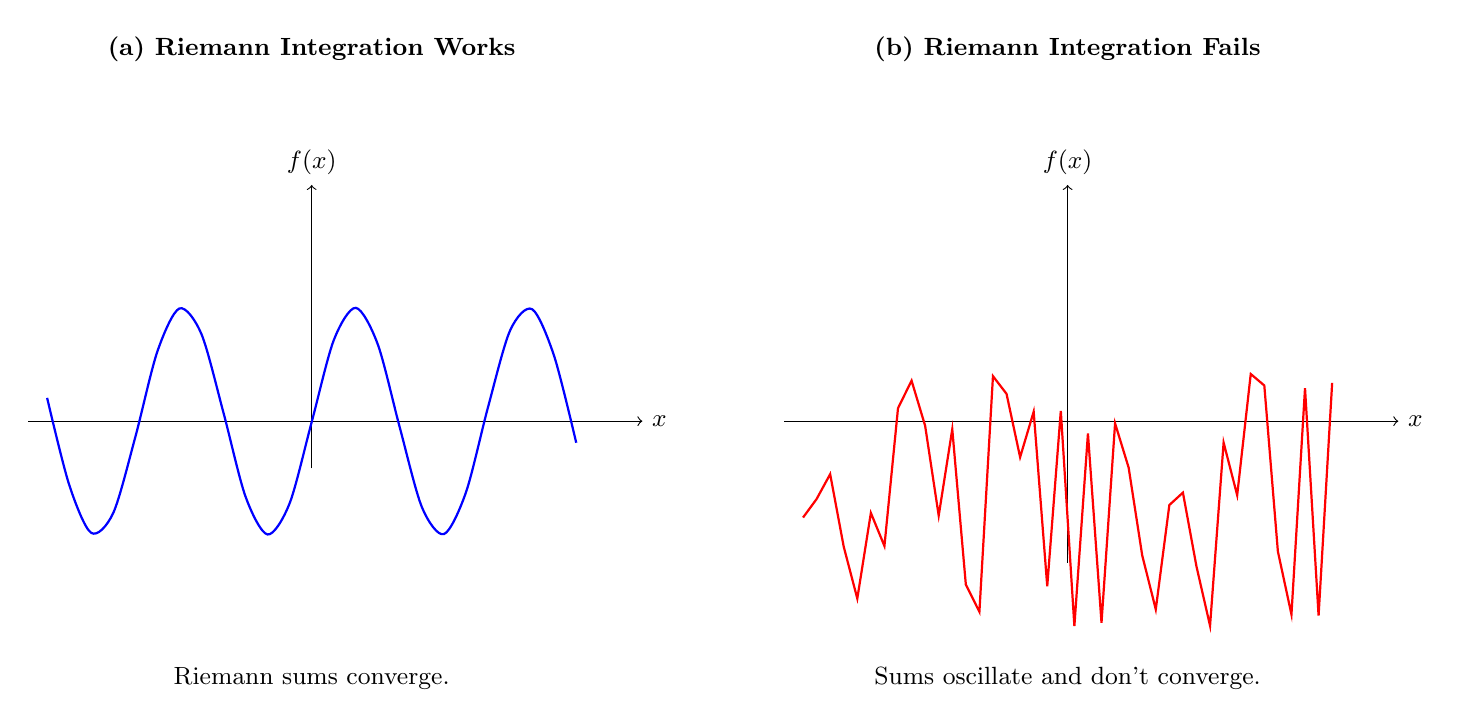
\begin{tikzpicture}[scale=1.2]

        % ---------------- Well-Behaved Function (Left Graph) ---------------- 
        \begin{scope}[shift={(0,0)}]

            % Axes
            \draw[->] (-3,0) -- (3.5,0) node[right] {\small $x$};
            \draw[->] (0,-0.5) -- (0,2.5) node[above] {\small $f(x)$};

            % Smooth function curve
            \draw[thick, domain=-2.8:2.8, smooth, variable=\x, blue] plot ({\x}, {1.2*sin(deg(\x r))}) node[right] {};



            % Labels
            \node[above] at (0,3.7) {\small \textbf{(a) Riemann Integration Works}};
            \node[below] at (0,-2.5) {\small Riemann sums converge.};
        \end{scope}

        % ---------------- Irregular Function (Right Graph) ---------------- 
        \begin{scope}[shift={(8,0)}]

            % Axes
            \draw[->] (-3,0) -- (3.5,0) node[right] {\small $x$};
            \draw[->] (0,-1.5) -- (0,2.5) node[above] {\small $f(x)$};

            % Oscillating function
            \draw[thick, red, domain=-2.8:2.8, samples=40] plot (\x, {rand*1.5-0.75}) node[right] {};



            % Labels
            \node[above] at (0,3.7) {\small \textbf{(b) Riemann Integration Fails}};
            \node[below] at (0,-2.5) {\small Sums oscillate and don’t converge.};
        \end{scope}

    \end{tikzpicture}
    \caption{Comparison of Riemann Integration for Well-Behaved vs. Irregular Functions. (a) Smooth functions converge nicely under Riemann sums. (b) Irregular functions can fail to yield a proper integral.}
\end{figure}



\subsection{Riemannian Metric: The Dot Product Evolves}

Hamilton gave us a way to think of motion as geometry. His reformulation of mechanics turned trajectories into flows and forces into structure. In doing so, he made the \textbf{dot product}—a way of comparing direction and change—the central actor in understanding dynamics.

But in Hamilton’s world, space was still flat. The dot product was fixed. Motion unfolded on a smooth, Euclidean stage.

\medskip

\textbf{Then came Riemann.}

In his revolutionary 1854 habilitation lecture, \textit{“On the Hypotheses Which Lie at the Foundations of Geometry,”} Bernhard Riemann proposed a stunning generalization:  
\textbf{What if the dot product itself could vary from point to point?}

\subsubsection*{From Dot Products to Riemannian Metrics}

In flat Euclidean space, the square of the infinitesimal distance between two points is given by:
\[
ds^2 = dx^2 + dy^2 + dz^2
\]
Which is really just a 3D dot product:
\[
ds^2 = \vec{dx} \cdot \vec{dx}
\]

Riemann generalized this idea by replacing the standard dot product with a position-dependent version. In coordinates \( x^1, x^2, \dots, x^n \), he defined:
\[
ds^2 = \sum_{i,j=1}^n g_{ij}(x) \, dx^i dx^j
\]

The functions \( g_{ij}(x) \) define the \textbf{metric tensor}—a generalized, localized dot product that varies across the manifold. At each point, it tells you how to compare directions: how to measure length, angle, and curvature.

This was no longer a single universal dot product—it was a field of dot products. Geometry had gone dynamic.

\subsubsection*{Geometry as Local Comparison}

What Hamilton treated as a static structure—momentum, energy, alignment—Riemann treated as a fluid geometry:

\begin{itemize}
  \item Instead of one way to measure direction and distance, there were infinitely many—one at each point.
  \item Instead of a single coordinate grid, space itself could stretch, shear, and curve.
  \item Instead of treating the dot product as fixed, Riemann made it contextual—a local rulebook for each patch of the manifold.
\end{itemize}

\textbf{Every dot product was now a question: “How does space behave \textit{here}?”}

\subsubsection*{From Measurement to Motion: A New Stage for Descent}

The power of Riemann’s metric was not just in describing geometry—it was in guiding motion.  
The metric tells us how steep a slope is. How far a step moves.  
In essence: \textbf{how change feels locally}.

This is the exact intuition behind \textbf{gradient descent}:

\begin{quote}
To move “downhill” in a curved space, you need to know which direction is steepest—and that depends on the local dot product.
\end{quote}

On a Riemannian manifold, the gradient of a function \( f \) is not just the vector of partial derivatives. It is the vector that, under the metric \( g \), points in the direction that maximally increases \( f \):
\[
\text{grad}_g f \quad \text{is the unique vector such that} \quad g(\text{grad}_g f, v) = df(v) \quad \forall v
\]

This equation is a dot product—but now one defined by the metric tensor \( g \). It is the Riemannian generalization of Hamilton’s core idea: use a directional product to measure how change aligns with motion.

\begin{tcolorbox}[colback=blue!5!white, colframe=blue!50!black,
title={Sidebar: Hamilton’s Dot Product Grows Up}]
Hamilton introduced the dot product as a tool for measuring projection, alignment, and energy.

Riemann turned that dot product into a \textbf{field}—a geometry where every point has its own rulebook for measurement.

Together, they gave us the key to modern optimization:
\begin{itemize}
  \item Measure alignment (Hamilton)
  \item Let that measurement depend on context (Riemann)
  \item Use it to move efficiently through space (Gradient Descent)
\end{itemize}
\end{tcolorbox}

\subsubsection*{A Geometry of Descent}

By unifying dot products with curvature, Riemann made it possible to define gradients and descent directions on curved spaces—on manifolds of shapes, probabilities, or quantum states.

\begin{quote}
Just as Hamilton revealed the symphony behind motion,  
Riemann gave us the score paper: a flexible sheet that bends, stretches, and curves—guiding every note of change.
\end{quote}

Later, when we study gradient descent and machine learning on manifolds, we’ll see Riemann’s influence again:  
\textbf{To find the optimal path, you don’t just follow the slope—you follow the slope that’s defined by the geometry beneath your feet.}
